\documentclass[10pt]{article}

\usepackage{preprint}
\usepackage{amsmath}
\usepackage{graphicx}
\usepackage{booktabs}
\usepackage{tabularx}
\usepackage{array}
\usepackage{colortbl}
\usepackage{float}
% Floats stay in the section that discusses them (placeins), and try "here" first.
\usepackage[section]{placeins}
\usepackage[labelformat=parens,labelsep=space]{subcaption}
\usepackage{tikz}
\usetikzlibrary{arrows.meta,positioning,calc,fit,backgrounds}
\usepackage{pgfplots}
\pgfplotsset{compat=1.18}
\usepackage[numbers,sort&compress]{natbib}
\usepackage{hyperref}
\usepackage{url}
\usepackage{xurl}

\definecolor{linkblue}{RGB}{0,20,115}
\definecolor{urlmag}{RGB}{160,40,120}
\hypersetup{colorlinks=true,linkcolor=linkblue,citecolor=linkblue,urlcolor=urlmag}

% ------------------------------------------------------------------------------
% Palette: the demo's tokens (web/src/styles/tokens.css). Data colours are the sensor-group
% colours, validated for colour-vision deficiency in this order; red is only the alarm.
% ------------------------------------------------------------------------------
\definecolor{ink}{HTML}{15212A}
\definecolor{ink2}{HTML}{56636E}
\definecolor{line}{HTML}{D3DAE0}
\definecolor{accent}{HTML}{2D6FA6}
\definecolor{accentsoft}{HTML}{EEF1F3}
\definecolor{ok}{HTML}{1B6E3A}
\definecolor{fault}{HTML}{C62828}
\definecolor{dblue}{HTML}{3D8FD1}
\definecolor{dbrown}{HTML}{A0561A}
\definecolor{dgreen}{HTML}{1F8A70}
\definecolor{dviolet}{HTML}{7B4FA8}
\definecolor{dgrey}{HTML}{9AA6B0}

\pgfplotsset{
  every axis/.append style={width=\linewidth, height=4.6cm, grid=major, grid style={line, line width=0.3pt},
    tick label style={font=\scriptsize}, label style={font=\scriptsize}, legend style={font=\scriptsize, draw=line, fill=white, fill opacity=0.9, text opacity=1},
    axis line style={ink2}, every axis plot/.append style={line width=0.9pt},
    /pgf/number format/1000 sep={}},
}

% Let a large figure sit under the text that introduces it instead of floating to its own page.
\renewcommand{\topfraction}{0.85}
\renewcommand{\bottomfraction}{0.6}
\renewcommand{\textfraction}{0.1}
\renewcommand{\floatpagefraction}{0.8}

\graphicspath{{./figures/}}
\newcommand{\kf}{Keyframe}
% The keyframe diamond: hollow for the fault switch-on, filled red for the alarm.
\DeclareRobustCommand{\switchmark}{\tikz[baseline=-0.6ex]\draw[ink, line width=0.6pt, fill=white] (0,0.09) -- (0.09,0) -- (0,-0.09) -- (-0.09,0) -- cycle;}
\DeclareRobustCommand{\alarmmark}{\tikz[baseline=-0.6ex]\fill[fault] (0,0.09) -- (0.09,0) -- (0,-0.09) -- (-0.09,0) -- cycle;}
% Table rows from a generated file: the primitive input is safe inside tabular.
\makeatletter\newcommand{\inputrows}[1]{\@@input #1 }\makeatother
% Generated by paper/make_data.py from the locked results. Do not edit.
\newcommand{\DataRowsModelling}{107,979}
\newcommand{\DataRowsAll}{114,770}
\newcommand{\DataRowsReference}{25,302}
\newcommand{\DataRowsLockbox}{6,791}
\newcommand{\DataFaultRuns}{14}
\newcommand{\DataHealthyMinMin}{28}
\newcommand{\DataHealthyMinMax}{111}
\newcommand{\DataFaultyMinMin}{66}
\newcommand{\DataFaultyMinMax}{129}
\newcommand{\DataRunsWithSwitchOn}{13}
\newcommand{\FeatCount}{833}
\newcommand{\ExportAlarmDuration}{45}
\newcommand{\ExportAlarmProbability}{0.7}
\newcommand{\BaseMajority}{0.108}
\newcommand{\BaseLogreg}{0.440}
\newcommand{\BaseLogregFar}{22.5}
\newcommand{\BaseLightgbm}{0.389}
\newcommand{\BaseForest}{0.285}
\newcommand{\LockShare}{100}
\newcommand{\LockLabel}{injector nozzle clogging}
\newcommand{\CrossMin}{0.07}
\newcommand{\CrossMax}{0.29}
\newcommand{\LatPredict}{91}
\newcommand{\LatExplain}{148}
\newcommand{\LatWindow}{600}
\newcommand{\AblRaw}{0.389}
\newcommand{\AblPhysics}{0.572}
\newcommand{\AblRolling}{0.617}
\newcommand{\AblRollingFar}{8.5}
\newcommand{\AblResidualBest}{0.608}
\newcommand{\AblPruned}{0.558}
\newcommand{\AblShopMain}{0.608}
\newcommand{\AblShopTest}{0.587}
\newcommand{\ModelsSecond}{0.667}
\newcommand{\AnomAuroc}{0.528}
\newcommand{\CalEce}{0.176}
\newcommand{\CalEceEightyFive}{0.499}
\newcommand{\PhysPassed}{2}
\newcommand{\SensDropped}{40}
\newcommand{\SensFForty}{0.635}
\newcommand{\SensFSixty}{0.725}
\newcommand{\SensFSeventyFive}{0.611}
\newcommand{\SensFEightyFive}{0.347}
\newcommand{\SensCwBefore}{0.96}
\newcommand{\SensCwAfter}{0.00}
\newcommand{\SensAfBefore}{0.25}
\newcommand{\SensAfAfter}{0.80}
\newcommand{\ReplaySwitchMin}{43.7}
\newcommand{\ReplayAlarmMin}{46.8}
\newcommand{\ReplayDelay}{3\,min 9\,s}
\newcommand{\ResFOne}{0.717}
\newcommand{\ResAccuracy}{0.761}
\newcommand{\ResFar}{12.2}
\newcommand{\ResWorstRecall}{0.194}
\newcommand{\TuneTrialsMin}{8}
\newcommand{\TuneTrialsMax}{9}
\newcommand{\FoldFForty}{0.547}
\newcommand{\FoldFarForty}{9.9}
\newcommand{\FoldFSixty}{0.860}
\newcommand{\FoldFarSixty}{7.6}
\newcommand{\FoldFSeventyFive}{0.701}
\newcommand{\FoldFarSeventyFive}{25.3}
\newcommand{\FoldFEightyFive}{0.609}
\newcommand{\FoldFarEightyFive}{9.7}
\newcommand{\FoldSpreadMin}{0.547}
\newcommand{\FoldSpreadMax}{0.860}
\newcommand{\ResFOneAfterTen}{0.725}
\newcommand{\AlarmRuns}{13}
\newcommand{\AlarmDetected}{6}
\newcommand{\AlarmMissed}{7}
\newcommand{\AlarmMedian}{9\,min 23\,s}
\newcommand{\AlarmMedianS}{563}
\newcommand{\AlarmFastest}{3\,min 7\,s}
\newcommand{\AlarmSlowest}{91\,min 25\,s}

% Generated by paper/make_data.py from the locked results. Do not edit.
\newcommand{\TestsPython}{185}
\newcommand{\TestsWeb}{110}


\title{\kf: Fault Diagnosis for a Marine Diesel Engine, Scored on Engine Loads the Model Never Saw}
\author{FNM}
\affiliation{Independent project}

\begin{document}

\maketitle

\begin{abstract}
Engine-room alarm systems mostly trip when one reading crosses a fixed limit, by which time a fault is usually well developed. A model that reads the pattern across many sensors could flag a fault earlier and name its cause, but models trained on synthetic engine data can score well without learning how an engine behaves. We present \kf{}, a fault classifier for a marine diesel trained on real test-bench data: \DataFaultRuns{} runs of five faults at 40 to 85\,\% load, most with the fault switched on partway through, plus healthy reference running. Every score comes from a model that never saw the engine load it is tested on, with hyperparameters and alarm settings chosen inside the training loads, and the targets and an engineering checklist of what each fault should do to the sensors were fixed before any model saw the data. The best model, XGBoost on raw readings, physics features and rolling windows, reaches a macro F1 of \ResFOne{} (target 0.80), with a false alarm rate of \ResFar\,\% and a sustained alarm on \AlarmDetected{} of \AlarmRuns{} fault runs. Two of nine targets are met. SHAP explanations match the engineering checklist for air cooler fouling and injector clogging, but air filter clogging and cooling water pump cavitation are partly recognised by channels that drift with the test day: without them, cavitation recall at 60\,\% load falls from \SensCwBefore{} to \SensCwAfter. A browser demo replays each run with the evaluated predictions and alarms. Every number and plot in this paper is generated from the locked results files.
\end{abstract}

% ==============================================================================
\section{Introduction}
% ==============================================================================

A marine diesel is monitored by dozens of sensors: charge air pressure and temperature, exhaust temperature per cylinder and around the turbocharger, cooling water and lube oil temperatures, pressures and flows, fuel flow and shaft power. The alarm and monitoring system compares most of them with fixed limits. A fault such as a fouling charge air cooler shows up first as a small, consistent shift across several related readings, and reaches a limit only much later~\cite{heywood1988}. A model that reads all the sensors together could raise the alarm sooner and name the likely cause.

This project follows an earlier one that trained a fault model on a synthetic engine dataset. Synthetic engine data tends to be generated as independent noise per sensor with each fault added as a fixed offset; the dataset used there had no correlation between sensors above 0.04, no link between one reading and the next, and faults lasting one second. A model can score well on such data without learning anything about engines. The Marine Engine Fault Dataset~\cite{bahootoroody2026dataset,bahootoroody2026descriptor} records a real marine diesel on a test bench, where healthy readings hold together physically and each fault develops over two to three hours.

Real data brings a harder problem: honest evaluation. Readings two seconds apart are nearly identical, so a random train-test split scores close to perfect while measuring nothing~\cite{kaufman2012leakage,roberts2017cv}. The question that matters to an engine maker is whether the model works at an operating point it has not seen. \kf{} answers that question and reports what it finds, including where it fails. Our contributions are:
\begin{itemize}
  \item A \textbf{leakage-controlled evaluation} on real bench data: leave-one-load-out validation with nested tuning, alarm settings chosen inside the training loads, targets and an engineering checklist fixed before modelling, and a lockbox run scored once (Section~\ref{sec:protocol}).
  \item \textbf{Results reported as they came out}, including the targets missed and a sensitivity analysis showing which part of the score comes from recognising the test day rather than the fault (Sections~\ref{sec:results} and~\ref{sec:explain}).
  \item A \textbf{physics check of the explanations}: the top SHAP features of each fault compared with the pre-registered checklist (Section~\ref{sec:explain}).
  \item A \textbf{browser demo} that replays each run with the evaluated predictions, alarms and explanations, and a what-if view backed by an API (Section~\ref{sec:demo}).
\end{itemize}

\begin{figure}[!htbp]
\centering
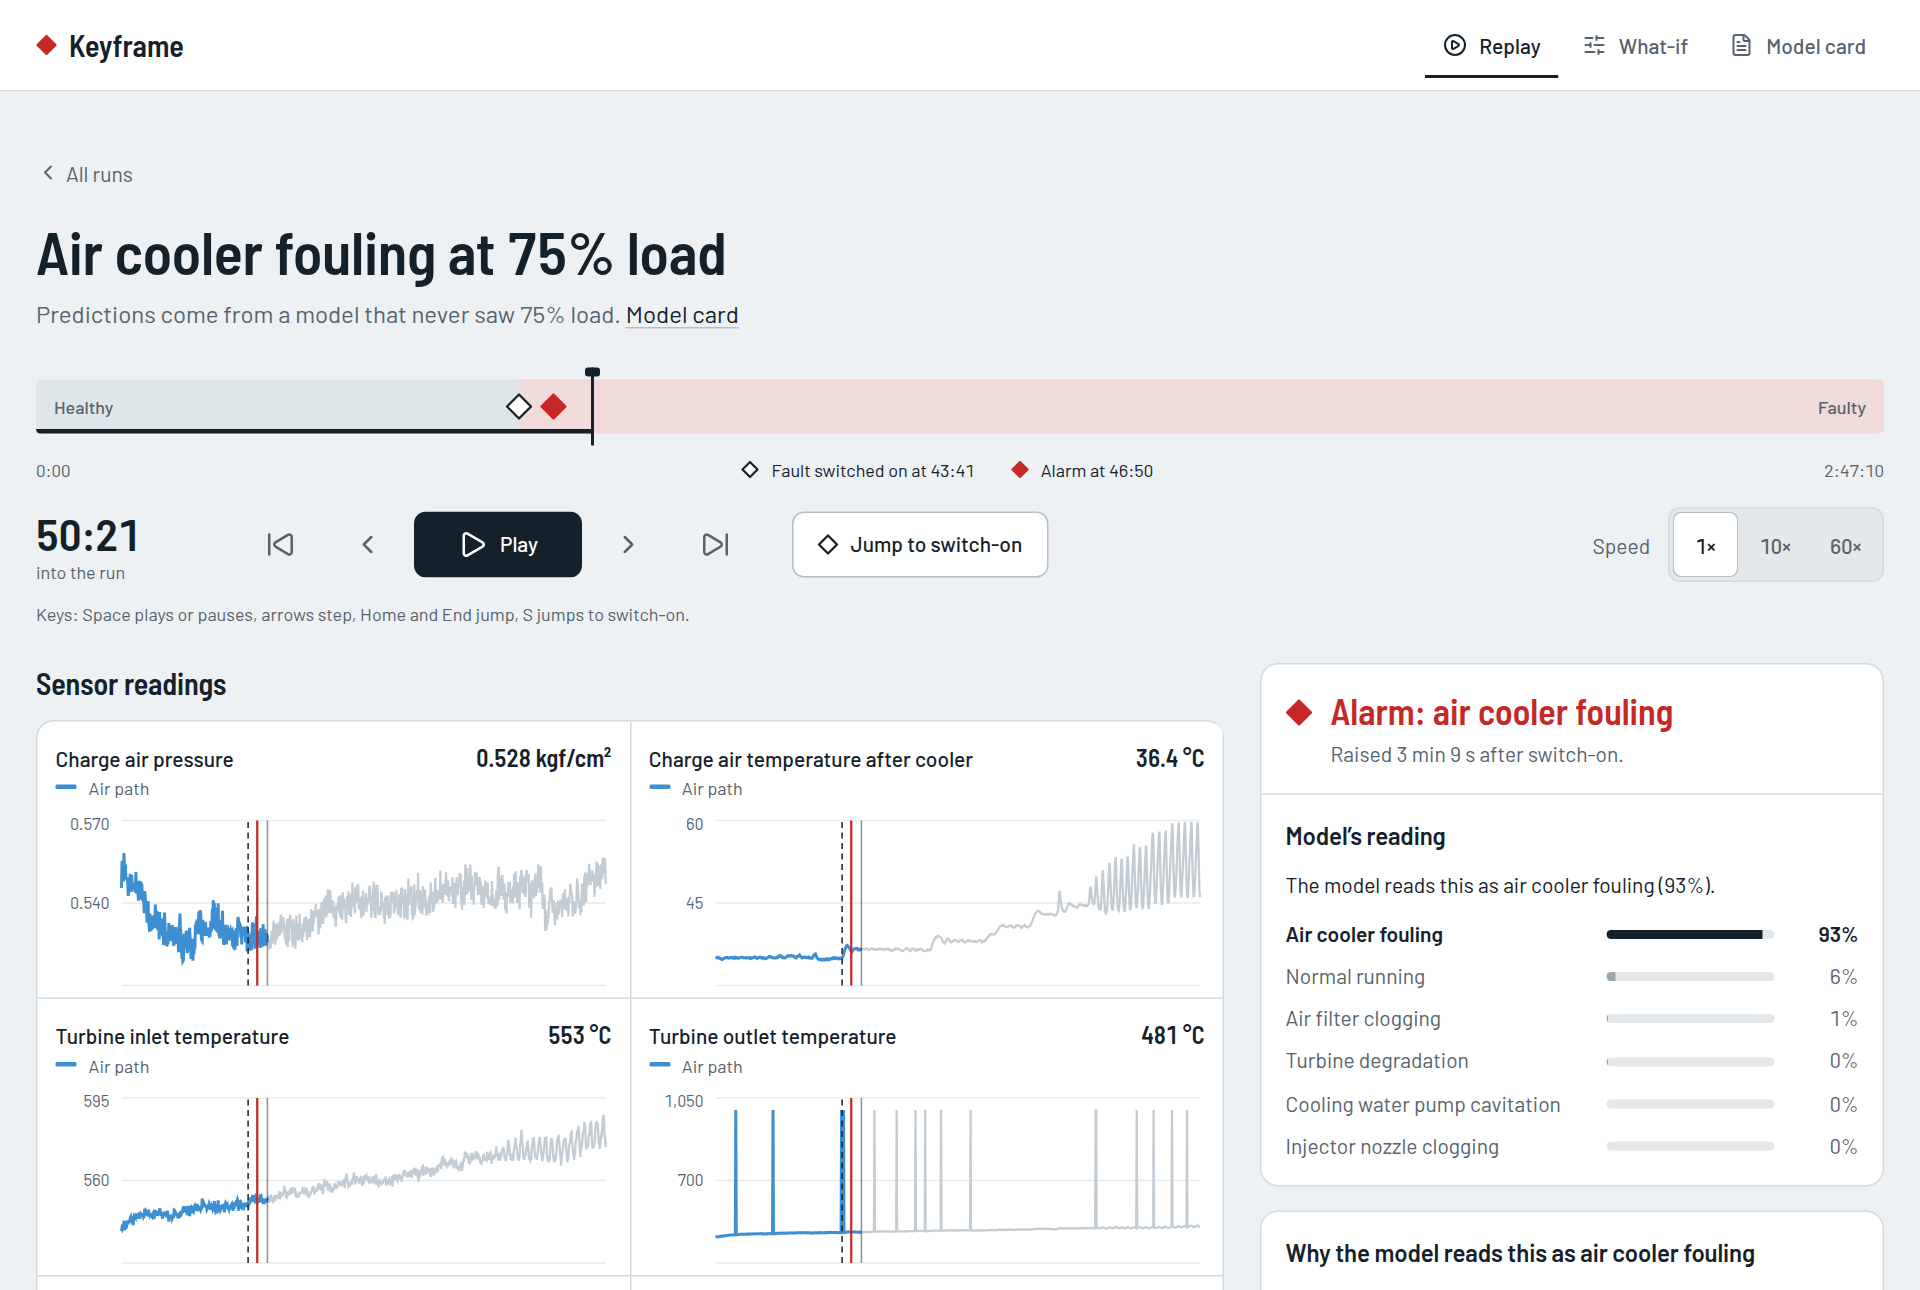
\includegraphics[width=\textwidth]{demo-replay}
\caption{\textbf{The replay view, air cooler fouling at 75\,\% load.} The timeline under the title is also the scrubber: grey is healthy running, red is the faulty stretch, the hollow diamond \switchmark{} marks the fault switch-on and the red diamond \alarmmark{} the alarm. The predictions come from the model trained without 75\,\% load. Trend charts are grouped and coloured by sensor group; the panel on the right states whether the alarm has fired and what the model reads.}
\label{fig:hero}
\end{figure}

% ==============================================================================
\section{Data}
% ==============================================================================

The Marine Engine Fault Dataset v1.0~\cite{bahootoroody2026dataset} was recorded on a Matsui Iron Works MU323DGSC three-cylinder marine diesel on a water-brake test bench. It holds 16 files and \DataRowsAll{} rows logged every one to two seconds. \DataRunsWithSwitchOn{} of the \DataFaultRuns{} fault runs hold the engine at one load, start healthy, and switch one fault on once; the healthy stretch lasts \DataHealthyMinMin{} to \DataHealthyMinMax{} minutes and the faulty stretch \DataFaultyMinMin{} to \DataFaultyMinMax{} minutes. A separate reference file holds \DataRowsReference{} rows of healthy running across the load range. Table~\ref{tab:coverage} lists the runs.

\begin{table}[!htbp]
\caption{\textbf{Rows per fault and load.} The injector run steps through 40, 60 and 85\,\% load with a brief stay at 75\,\%, and is faulty from its first row. A second injector run, with two nozzle holes plugged, is set aside as the lockbox (\DataRowsLockbox{} rows).}
\label{tab:coverage}
\centering\small
\begin{tabular}{@{}lrrrr@{}}
\toprule
Fault (what was done to the engine) & 40\,\% & 60\,\% & 75\,\% & 85\,\% \\
\midrule
\inputrows{data/coverage.tex}
\bottomrule
\end{tabular}
\end{table}

The faults are air cooler fouling (charge air cooling degraded), air filter clogging (compressor inlet covered step by step), injector nozzle clogging (one hole plugged in one cylinder), cooling water pump cavitation (air injected at the pump suction) and turbine degradation (exhaust back pressure raised after the turbine). Coverage is uneven: cavitation was run only at 60 and 85\,\% load, turbine degradation not at 75\,\%.

A data audit (notebook 00) found three things that shape the evaluation. First, two channels record the researchers' own set points for the air filter and turbine faults, the knobs they turned to create the fault, and are empty in several runs; they are dropped, since a model that reads them is reading the answer. Second, the engine room temperature and other slowly drifting channels differ by test day, so a model could learn which day a run was recorded on; these channels are kept but tested for (Section~\ref{sec:explain}). Third, the switch-on point of each run is taken from the labels and plotted against the sensors. Figure~\ref{fig:switchon} shows the signature an engineer would expect for air cooler fouling: the air temperature after the cooler steps up at switch-on and keeps rising.

\begin{figure}[!htbp]
\centering
\begin{tikzpicture}
\begin{axis}[xlabel={Minutes from fault switch-on}, ylabel={Charge air temp.\ after cooler ($^\circ$C)}, xmin=-30, xmax=60, legend style={at={(0.5,1.03)}, anchor=south}, legend columns=4, unbounded coords=jump, height=5cm]
\addplot[dblue] table[x=t_min, y=l40, col sep=comma] {data/switchon_ac.csv};
\addplot[dbrown] table[x=t_min, y=l60, col sep=comma] {data/switchon_ac.csv};
\addplot[dgreen] table[x=t_min, y=l75, col sep=comma] {data/switchon_ac.csv};
\addplot[dviolet] table[x=t_min, y=l85, col sep=comma] {data/switchon_ac.csv};
\legend{40\,\%, 60\,\%, 75\,\%, 85\,\%}
\draw[ink, densely dashed] ({axis cs:0,0} |- {rel axis cs:0,0}) -- ({axis cs:0,0} |- {rel axis cs:0,1});
\end{axis}
\end{tikzpicture}
\caption{\textbf{Air cooler fouling around its switch-on}, at each load (30-second means). The dashed line is the switch-on. At 40\,\% load the outlet temperature cycles strongly before and after the switch-on, which hides the step; this is also the run the model detects last.}
\label{fig:switchon}
\end{figure}

% ==============================================================================
\section{Evaluation protocol}
\label{sec:protocol}
% ==============================================================================

\subsection{Leave one load out, with nested tuning}

Every score comes from a model that never saw the engine load it is tested on (Figure~\ref{fig:lolo}). The four load bins, 40, 60, 75 and 85\,\%, give four outer folds. Inside each outer fold, the three training loads form inner folds in the same way, and everything that is chosen, hyperparameters, feature pruning and alarm settings, is chosen on those inner folds only~\cite{varma2006bias}. Healthy-engine models used for residual features are fitted on the training loads' healthy rows only. Scores are pooled over the four held-out loads and reported per load, because the spread between loads is part of the result.

\begin{figure}[!htbp]
\centering
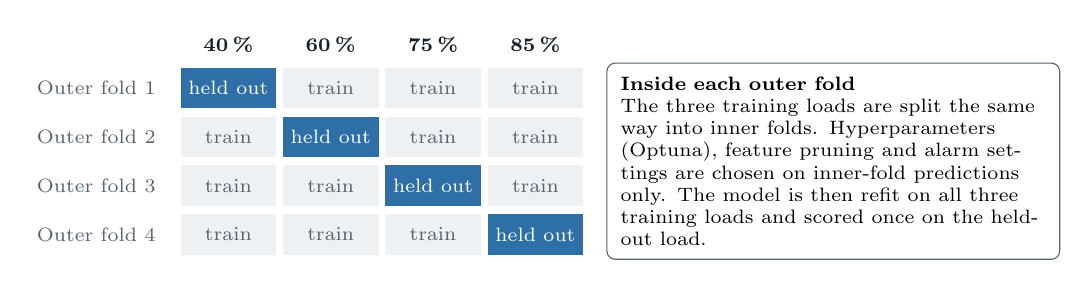
\begin{tikzpicture}[
  cell/.style={draw=white, line width=1pt, minimum width=1.25cm, minimum height=0.55cm, font=\scriptsize, inner sep=0pt},
  train/.style={cell, fill=accentsoft, text=ink2},
  test/.style={cell, fill=accent, text=white},
  lab/.style={font=\scriptsize, text=ink2, anchor=east},
]
\foreach \load [count=\i] in {40,60,75,85} {
  \node[font=\scriptsize\bfseries, text=ink] at (\i*1.3, 0.55) {\load\,\%};
}
\foreach \held [count=\row] in {40,60,75,85} {
  \node[lab] at (0.5, -\row*0.62+0.62) {Outer fold \row};
  \foreach \load [count=\i] in {40,60,75,85} {
    \ifnum\load=\held
      \node[test] at (\i*1.3, -\row*0.62+0.62) {held out};
    \else
      \node[train] at (\i*1.3, -\row*0.62+0.62) {train};
    \fi
  }
}
\node[draw=ink2, rounded corners=3pt, align=left, font=\scriptsize, text width=5.4cm, anchor=west, inner sep=5pt] (inner) at (6.1, -0.93) {\textbf{Inside each outer fold}\\The three training loads are split the same way into inner folds. Hyperparameters (Optuna), feature pruning and alarm settings are chosen on inner-fold predictions only. The model is then refit on all three training loads and scored once on the held-out load.};
\end{tikzpicture}
\caption{\textbf{Leave-one-load-out validation with nested selection.} No choice sees the held-out load. Random row splits are never used: they place near-identical readings on both sides and score close to 1.00.}
\label{fig:lolo}
\end{figure}

\subsection{Fixed in advance}

Nine targets were set in the project brief before any modelling, from a first baseline, and reviewed once after the exploratory analysis without change. An engineering checklist of what each fault should do to each sensor group, based on engine physics~\cite{heywood1988}, was written during the exploratory analysis and pinned by its SHA-256 hash before any model saw the data, in the spirit of pre-registration~\cite{nosek2018prereg}; a test fails if it changes. A second injector run, with two nozzle holes plugged instead of one, was moved aside at download as a lockbox and scored once, after every choice was fixed. Results were then locked, and later defects were recorded rather than fixed in place.

\subsection{Measures}

Macro F1 is the unweighted mean of per-class F1 over the six classes (normal running and five faults). The false alarm rate is the share of truly healthy rows predicted as any fault. An alarm is \emph{sustained}: a fault class is active once every prediction over the trailing $d$ seconds of a run is that class with probability at least $p$. The pair $(d,p)$ is chosen per outer fold by a grid search over $d \in \{30, 60, 120, 300\}$\,s and $p \in \{0.5, 0.6, 0.7, 0.8\}$ on inner-fold predictions, taking the lowest median detection delay among settings whose alarm-level false alarm rate is at most 5\,\%. Detection delay is the time from switch-on to the first alarm. Expected calibration error (ECE) uses 15 confidence bins~\cite{naeini2015ece}. Anomaly detectors are scored by the area under the ROC curve (AUROC) for faulty against healthy rows.

% ==============================================================================
\section{Features and models}
% ==============================================================================

\paragraph{Feature sets.} Four families were compared in an ablation (Table~\ref{tab:ablation}). \emph{Raw readings} are the sensor channels after the audit. \emph{Physics features} are quantities an engineer would compute, for example compressor pressure ratio, charge air cooler effectiveness, exhaust temperature spread and each cylinder's deviation from the mean, turbine temperature drop, peak pressure and indicated work spread between cylinders, fuel flow per kilowatt, and the share of heat rejected to each cooling circuit. \emph{Residuals} are each channel minus what a healthy engine would read at the same operating point, predicted by a degree-2 polynomial ridge regression from engine speed, brake load and fuel flow, fitted on healthy training rows only; a polynomial rather than trees, because the 40 and 85\,\% held-out loads sit at the edges of the training range. \emph{Rolling windows} add causal mean, spread and trend over the last 60, 300 and 900 seconds of each run.

\begin{table}[!htbp]
\caption{\textbf{Feature ablation}, pooled over the four held-out loads (untuned models). Physics features and rolling windows earn their place with the tree model; residuals help the linear model but not the trees. FAR is the false alarm rate in \%.}
\label{tab:ablation}
\centering\small
\begin{tabular}{@{}lrrrr@{}}
\toprule
 & \multicolumn{2}{c}{Logistic regression} & \multicolumn{2}{c}{LightGBM} \\
\cmidrule(lr){2-3}\cmidrule(l){4-5}
Feature set & Macro F1 & FAR & Macro F1 & FAR \\
\midrule
\inputrows{data/ablation.tex}
\bottomrule
\end{tabular}
\end{table}

The first baseline, logistic regression on raw readings, scored \BaseLogreg{} against \BaseMajority{} for always predicting the majority class. With LightGBM, macro F1 rises from \AblRaw{} on raw readings to \AblPhysics{} with physics features and \AblRolling{} with rolling windows, while the false alarm rate falls to \AblRollingFar\,\%. Pruning correlated features inside each training fold lowered the score (\AblPruned), so the unpruned raw, physics and rolling set, \FeatCount{} features, went forward. Letting the residual model also see the reference file's healthy rows at the held-out load, as a shop test before commissioning would provide, changed the best residual arm's score from \AblShopMain{} to \AblShopTest; it is reported but not used.

\paragraph{Models.} Four model families were tuned with Optuna~\cite{akiba2019optuna} inside each outer fold: logistic regression, random forest~\cite{pedregosa2011sklearn}, LightGBM~\cite{ke2017lightgbm} and XGBoost~\cite{chen2016xgboost}, all with balanced class weights. Table~\ref{tab:models} compares them. XGBoost is best on macro F1 and is the model reported from here on; its false alarm rate is higher than LightGBM's.

\begin{table}[!htbp]
\caption{\textbf{Tuned models}, pooled over the four held-out loads. Worst recall is the lowest per-class recall, with its class.}
\label{tab:models}
\centering\small
\begin{tabular}{@{}lrrrl@{}}
\toprule
Model & Macro F1 & Accuracy & FAR (\%) & Worst recall \\
\midrule
\inputrows{data/models.tex}
\bottomrule
\end{tabular}
\end{table}

Tuning ran on a time budget per fold, and each XGBoost search finished only \TuneTrialsMin{} to \TuneTrialsMax{} trials (Table~\ref{tab:hyper}). The sampler is seeded, so the folds propose the same candidates, and the 40 and 60\,\% folds settled on the same one. The 85\,\% fold settled on a learning rate of 0.0034 with 59 trees, which barely moves the model from its prior: its highest class probability on any held-out row is 0.26. This was found after the results were locked and is reported rather than re-tuned, because re-tuning after seeing held-out predictions would select on the test folds.

\begin{table}[!htbp]
\caption{\textbf{XGBoost settings chosen per held-out load}, with the number of Optuna trials that finished and the held-out macro F1.}
\label{tab:hyper}
\centering\small
\begin{tabular}{@{}lrrrrrrr@{}}
\toprule
Held out & Learning rate & Trees & Depth & Subsample & Columns & Trials & Macro F1 \\
\midrule
\inputrows{data/hyperparameters.tex}
\bottomrule
\end{tabular}
\end{table}

% ==============================================================================
\section{Results}
\label{sec:results}
% ==============================================================================

Table~\ref{tab:targets} sets the results against the targets fixed in advance. Two of nine are met, and one of those, the lockbox, is weak evidence.

\begin{table}[!htbp]
\caption{\textbf{Targets and locked results}, pooled over the held-out loads.}
\label{tab:targets}
\centering\small
\begin{tabularx}{\textwidth}{@{}Xrrl@{}}
\toprule
Measure & Result & Target & \\
\midrule
Macro F1 & \ResFOne & 0.80 & not met \\
Lowest per-class recall (turbine degradation) & \ResWorstRecall & 0.70 & not met \\
False alarm rate & \ResFar\,\% & 5\,\% & not met \\
Detection delay, median of runs that alarmed & \AlarmMedian & 10\,min & not met (\AlarmDetected{} of \AlarmRuns{} runs alarm) \\
Fault detection AUROC, healthy-only detectors & \AnomAuroc & 0.95 & not met \\
Expected calibration error & \CalEce & 0.05 & not met \\
Lockbox labelled injector clogging & \LockShare\,\% & 90\,\% & met, weak evidence \\
Physics check on explanations & \PhysPassed{} of 5 & 4 of 5 & not met \\
Demo response, prediction plus explanation & \LatExplain\,ms & 300\,ms & met \\
\bottomrule
\end{tabularx}
\end{table}

\paragraph{Classification.} Pooled macro F1 is \ResFOne{} and accuracy \ResAccuracy. Scores swing with the held-out load, from \FoldSpreadMin{} to \FoldSpreadMax{} (Figure~\ref{fig:folds}). Excluding the first 10 minutes after each switch-on, when a fault has barely developed, raises macro F1 only to \ResFOneAfterTen, so the errors are not mainly early ones. The confusion matrix (Table~\ref{tab:confusion}) shows where they are: injector clogging and cavitation are almost always right, but most turbine degradation rows are read as normal running, and air filter clogging is split between normal running, air cooler fouling and itself.

\begin{table}[!htbp]
\caption{\textbf{Confusion matrix}, rows normalised to the true class, pooled over the four held-out loads. Shading follows the share.}
\label{tab:confusion}
\centering\small
\setlength{\tabcolsep}{5pt}
\begin{tabular}{@{}lcccccc@{}}
\toprule
True \textbackslash{} predicted & Normal & AC & AF & INJ & CW & TD \\
\midrule
\inputrows{data/confusion.tex}
\bottomrule
\end{tabular}
\end{table}

\paragraph{Alarms.} Table~\ref{tab:alarms} gives the alarm for every fault run with a switch-on. Of the \AlarmRuns{} runs, \AlarmDetected{} raise a sustained alarm, all naming the correct fault, after \AlarmFastest{} to \AlarmSlowest{} (median \AlarmMedian). None of the four runs at 85\,\% load alarms: the underfit 85\,\% model never reaches the probability its alarm setting requires. The settings chosen in the training loads differ widely between folds (Table~\ref{tab:alarmsettings}), which is itself a sign of how little data there is per load.

\begin{table}[!htbp]
\centering\small
\begin{minipage}[t]{0.58\textwidth}\centering
\caption{\textbf{Alarm per fault run}, from switch-on to the first sustained alarm. Every alarm names the fault that was switched on.}
\label{tab:alarms}
\begin{tabular}{@{}llr@{}}
\toprule
Fault & Load & Delay \\
\midrule
\inputrows{data/alarms.tex}
\bottomrule
\end{tabular}
\end{minipage}\hfill
\begin{minipage}[t]{0.38\textwidth}\centering
\caption{\textbf{Alarm settings} chosen in each fold's training loads: sustained seconds $d$, minimum probability $p$, and the alarm-level false alarm rate on the held-out load (\%).}
\label{tab:alarmsettings}
\begin{tabular}{@{}lrrr@{}}
\toprule
Held out & $d$ & $p$ & FAR \\
\midrule
\inputrows{data/alarm_settings.tex}
\bottomrule
\end{tabular}
\end{minipage}
\end{table}

Figure~\ref{fig:replay} follows the fastest detection, air cooler fouling at 75\,\% load. The model already gives air cooler fouling about 0.4 in the minutes before the switch-on, on a healthy engine, which is the kind of reading that produces false alarms. After the switch-on the cooler outlet temperature steps up, the probability passes 0.65 within a minute, and the alarm follows once it has held above the fold's threshold.

\begin{figure}[!htbp]
\centering
\begin{subfigure}[t]{0.49\textwidth}
\begin{tikzpicture}
\begin{axis}[xlabel={Minutes into the run}, ylabel={Charge air temp.\ after cooler ($^\circ$C)}, xmin=30, xmax=70]
\addplot[dblue] table[x=t_min, y=temp_c, col sep=comma] {data/replay_ac75.csv};
\draw[ink, densely dashed] ({axis cs:\ReplaySwitchMin,0} |- {rel axis cs:0,0}) -- ({axis cs:\ReplaySwitchMin,0} |- {rel axis cs:0,1});
\draw[fault] ({axis cs:\ReplayAlarmMin,0} |- {rel axis cs:0,0}) -- ({axis cs:\ReplayAlarmMin,0} |- {rel axis cs:0,1});
\end{axis}
\end{tikzpicture}
\caption{Cooler outlet air temperature.}
\end{subfigure}\hfill
\begin{subfigure}[t]{0.49\textwidth}
\begin{tikzpicture}
\begin{axis}[xlabel={Minutes into the run}, ylabel={Model probability}, xmin=30, xmax=70, ymin=0, ymax=1, legend style={at={(0.97,0.5)}, anchor=east}]
\addplot[ink] table[x=t_min, y=p_ac, col sep=comma] {data/replay_ac75.csv};
\addplot[dgrey] table[x=t_min, y=p_normal, col sep=comma] {data/replay_ac75.csv};
\legend{air cooler fouling, normal running}
\draw[ink, densely dashed] (axis cs:\ReplaySwitchMin,0) -- (axis cs:\ReplaySwitchMin,1);
\draw[fault] (axis cs:\ReplayAlarmMin,0) -- (axis cs:\ReplayAlarmMin,1);
\end{axis}
\end{tikzpicture}
\caption{Predicted probabilities.}
\end{subfigure}
\caption{\textbf{Air cooler fouling at 75\,\% load, as the demo replays it} (one frame every 10 seconds). The dashed line is the switch-on, the red line the alarm \ReplayDelay{} later.}
\label{fig:replay}
\end{figure}

\paragraph{Calibration and the lockbox.} Confidence is not reliable: pooled ECE is \CalEce{} (target 0.05). Temperature scaling~\cite{guo2017calibration}, fitted inside each fold's training loads, made calibration worse at three of four held-out loads (Table~\ref{tab:calibration}) and leaves predicted classes unchanged. On the lockbox, the two-hole injector run, \LockShare\,\% of rows were labelled \LockLabel, which meets the 90\,\% target; but no other class was predicted for that run at all, so it shows that the injector signature is strong, not that the model generalises to a more severe fault.

\begin{table}[!htbp]
\caption{\textbf{Calibration per held-out load}: ECE before and after temperature scaling with the temperature fitted in the training loads.}
\label{tab:calibration}
\centering\small
\begin{tabular}{@{}lrrr@{}}
\toprule
Held out & ECE before & Temperature & ECE after \\
\midrule
\inputrows{data/calibration.tex}
\bottomrule
\end{tabular}
\end{table}

\paragraph{Detection from healthy data alone.} Anomaly detectors trained only on healthy running, PCA reconstruction error, isolation forest~\cite{liu2008iforest} and an autoencoder, were scored on raw readings and on residuals, with the residual arm declared primary in advance. All are near chance (Table~\ref{tab:anomaly}); the headline AUROC is \AnomAuroc. They separate the injector fault best, whose cylinder imbalance is unusual at any load, and do no better than chance on cavitation.

\begin{table}[!htbp]
\caption{\textbf{Healthy-only anomaly detectors}, AUROC pooled over held-out loads, with the residual arm's AUROC for two faults.}
\label{tab:anomaly}
\centering\small
\begin{tabular}{@{}lrrrr@{}}
\toprule
Detector & Raw & Residual & Residual, INJ & Residual, CW \\
\midrule
\inputrows{data/anomaly.tex}
\bottomrule
\end{tabular}
\end{table}

% ==============================================================================
\section{Explanations and the physics check}
\label{sec:explain}
% ==============================================================================

Explanations use SHAP TreeExplainer~\cite{lundberg2017shap,lundberg2020tree} on each held-out load's model. Because rolling windows of one channel and the three cylinder temperatures move together, SHAP splits credit among them arbitrarily~\cite{aas2021shapley}, so we read SHAP summed within five sensor groups (Table~\ref{tab:groupedshap}) and by source channel, not single features. The groups are air path, fuel system, cooling, lube oil, and combustion and power; the demo colours them after ship pipework colour coding~\cite{iso14726}.

\begin{table}[!htbp]
\caption{\textbf{Mean SHAP per sensor group and fault class}, on each class's own held-out rows (log-odds). Bold marks the group that pushes most towards each class.}
\label{tab:groupedshap}
\centering\small
\begin{tabular}{@{}lrrrrr@{}}
\toprule
Group & AC & AF & INJ & CW & TD \\
\midrule
\inputrows{data/grouped_shap.tex}
\bottomrule
\end{tabular}
\end{table}

\paragraph{Physics check.} For each fault, the top five features by mean $|$SHAP$|$ were mapped to their source channels and compared with the checklist. A fault passes with at least three matches and no day-dependent channel in its top five (Table~\ref{tab:physics}). Air cooler fouling leans on the cooler outlet air temperature and injector clogging on the exhaust temperatures and their spread between cylinders, as the checklist predicted. Air filter clogging and cavitation lean on fuel temperatures, sea cooling water pressure and lube oil cooler water temperature, which drift with the test day. Turbine degradation leans on lube oil and efficiency channels rather than the turbine temperatures and pressures. Grouped by system, cavitation appears to rely on ``cooling'' (Table~\ref{tab:groupedshap}), but only because its shortcut channels sit in that group, so the grouped view alone would overstate agreement with the physics.

\begin{table}[!htbp]
\caption{\textbf{Physics check}: top-five features matching the pre-registered checklist, and whether a day-dependent channel is among them. \PhysPassed{} of 5 faults pass (target 4 of 5).}
\label{tab:physics}
\centering\small
\begin{tabular}{@{}lrll@{}}
\toprule
Fault & Matches & Day-dependent & Result \\
\midrule
\inputrows{data/physics.tex}
\bottomrule
\end{tabular}
\end{table}

\paragraph{Cross-checks.} Grouped permutation importance agrees only weakly with mean $|$SHAP$|$ (Spearman $r$ from \CrossMin{} to \CrossMax{} across folds), and LIME~\cite{ribeiro2016lime} shares about 2.7 of its top eight features with SHAP on one held-out moment per fault. We therefore treat the air cooler and injector stories as credible and the others as unconfirmed.

\paragraph{How much of the score is the test day?} Retraining the model without the \SensDropped{} features built from day-dependent channels tests the shortcut directly~\cite{geirhos2020shortcut}. Figure~\ref{fig:folds} shows the result. At 60\,\% load, cavitation recall falls from \SensCwBefore{} to \SensCwAfter: that run was recognised by its day, not its fault. At 40\,\% load the score rises and air filter clogging recall goes from \SensAfBefore{} to \SensAfAfter, so the day channels were also misleading the model there. The headline score is left as locked, and the model card states that part of it identifies the day.

\begin{figure}[!htbp]
\centering
\begin{tikzpicture}
\begin{axis}[ybar, bar width=0.42cm, ylabel={Macro F1}, xlabel={Held-out load (\%)}, symbolic x coords={40,60,75,85}, xtick=data, ymin=0, ymax=1, enlarge x limits=0.18, legend style={at={(0.5,1.03)}, anchor=south}, legend columns=2, height=5cm, width=0.8\linewidth, nodes near coords, nodes near coords style={font=\tiny, /pgf/number format/fixed, /pgf/number format/precision=2, /pgf/number format/fixed zerofill}]
\addplot[fill=accent, draw=accent] table[x=load, y=headline, col sep=comma] {data/sensitivity.csv};
\addplot[fill=dgrey, draw=dgrey] table[x=load, y=no_day, col sep=comma] {data/sensitivity.csv};
\legend{locked model, without day-dependent features}
\draw[fault, densely dashed] (rel axis cs:0,0.8) -- (rel axis cs:1,0.8) node[pos=0.02, anchor=south west, font=\tiny, text=fault] {target 0.80};
\end{axis}
\end{tikzpicture}
\caption{\textbf{Macro F1 per held-out load}, for the locked model and for the same model retrained without the \SensDropped{} day-dependent features. Removing them helps at 40\,\% load and hurts at the others, most at 85\,\%.}
\label{fig:folds}
\end{figure}

% ==============================================================================
\section{Demo and service}
\label{sec:demo}
% ==============================================================================

The results are meant to be judged by an engineer in a few minutes, so they ship with a browser demo (Figure~\ref{fig:arch}). An export step writes the final model, trained on all loads with the median of the per-fold hyperparameters, and one replay file per run: every tenth second of the run with the key sensor readings, the class probabilities, the alarm state and grouped SHAP values, all from the model that never saw that run's load. The replay and model card views are static files; the what-if view calls a FastAPI service that runs the exported model.

\begin{figure}[!htbp]
\centering
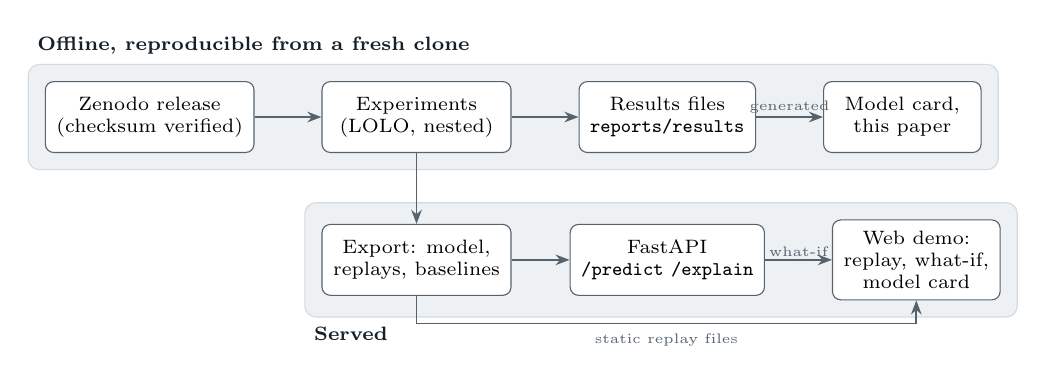
\begin{tikzpicture}[
  box/.style={draw=ink2, rounded corners=3pt, fill=white, align=center, font=\scriptsize, inner sep=4pt, minimum height=0.9cm},
  layer/.style={draw=line, rounded corners=4pt, fill=accentsoft, inner sep=6pt},
  lab/.style={font=\scriptsize\bfseries, text=ink, anchor=south west},
  arr/.style={-{Stealth[length=1.8mm]}, draw=ink2, line width=0.6pt},
]
\node[box, minimum width=2.2cm] (data) at (0,0) {Zenodo release\\(checksum verified)};
\node[box, minimum width=2.4cm, right=0.85cm of data] (exp) {Experiments\\(LOLO, nested)};
\node[box, minimum width=2.2cm, right=0.85cm of exp] (results) {Results files\\\texttt{reports/results}};
\node[box, minimum width=2.0cm, right=0.85cm of results] (paper) {Model card,\\this paper};
\node[box, minimum width=2.4cm, below=0.9cm of exp] (export) {Export: model,\\replays, baselines};
\node[box, minimum width=2.0cm, below=0.9cm of results] (api) {FastAPI\\\texttt{/predict} \texttt{/explain}};
\node[box, minimum width=2.0cm, right=0.85cm of api] (web) {Web demo:\\replay, what-if,\\model card};
\begin{scope}[on background layer]
\node[layer, fit=(data)(exp)(results)(paper)] (offline) {};
\node[layer, fit=(export)(api)(web)] (serve) {};
\end{scope}
\node[lab] at (offline.north west) {Offline, reproducible from a fresh clone};
\node[lab, anchor=north west] at (serve.south west) {Served};
\draw[arr] (data) -- (exp);
\draw[arr] (exp) -- (results);
\draw[arr] (results) -- node[above, font=\tiny, text=ink2, inner sep=1pt] {generated} (paper);
\draw[arr] (exp) -- (export);
\draw[arr] (export) -- (api);
\draw[arr] (api) -- node[above, font=\tiny, text=ink2, inner sep=1pt] {what-if} (web);
\draw[arr] (export.south) |- ++(0,-0.35) -| node[pos=0.25, below, font=\tiny, text=ink2] {static replay files} (web.south);
\end{tikzpicture}
\caption{\textbf{From data to demo.} Heavy experiments write results files; the model card, the demo's targets table and every number in this paper are generated from them, and tests fail if they drift.}
\label{fig:arch}
\end{figure}

Figure~\ref{fig:ui} shows three views. The runs table lists every run with a miniature timeline and its alarm delay. The replay (Figure~\ref{fig:hero}) plays a run at 1, 10 or 60 times real speed; pausing shows why the model reads the moment as it does, as a waterfall of grouped SHAP values in the sensor-group colours and the three strongest single readings in plain words. The what-if view starts from a healthy engine at one load, lets the user move any of ten readings, and shows the diagnosis and its explanation, assuming the readings have held steady for 15 minutes. The model card view opens with the targets table of Table~\ref{tab:targets}. A prediction takes \LatPredict\,ms and a prediction with its explanation \LatExplain\,ms (median, \LatWindow-row window).

\begin{figure}[!htbp]
\centering
\begin{subfigure}[t]{0.44\textwidth}\centering
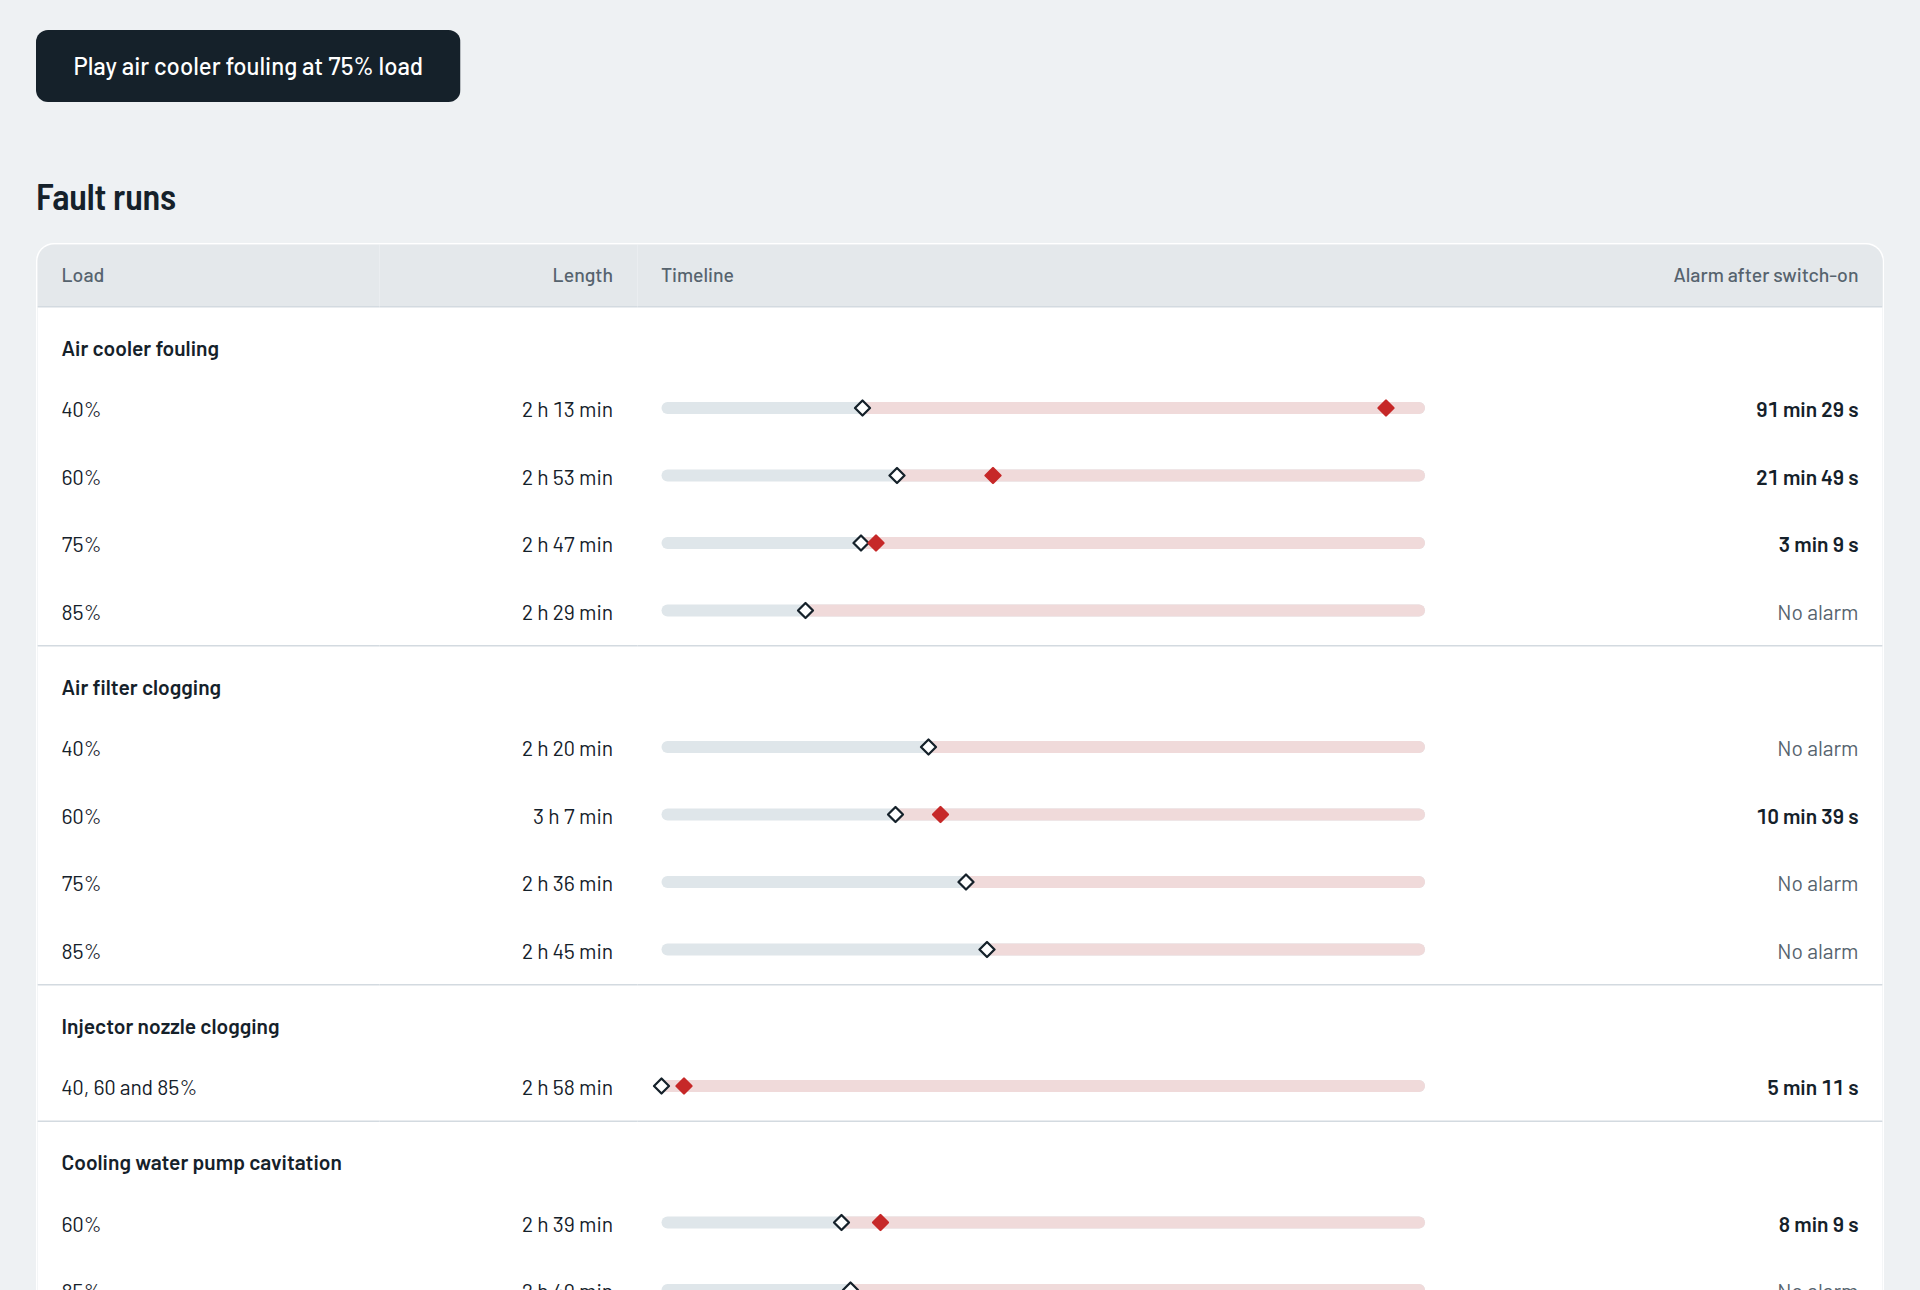
\includegraphics[width=\linewidth]{ui-runs}
\caption{Runs: a miniature keyframe timeline per run and the alarm delay on the right.}
\end{subfigure}\hspace{0.04\textwidth}
\begin{subfigure}[t]{0.44\textwidth}\centering
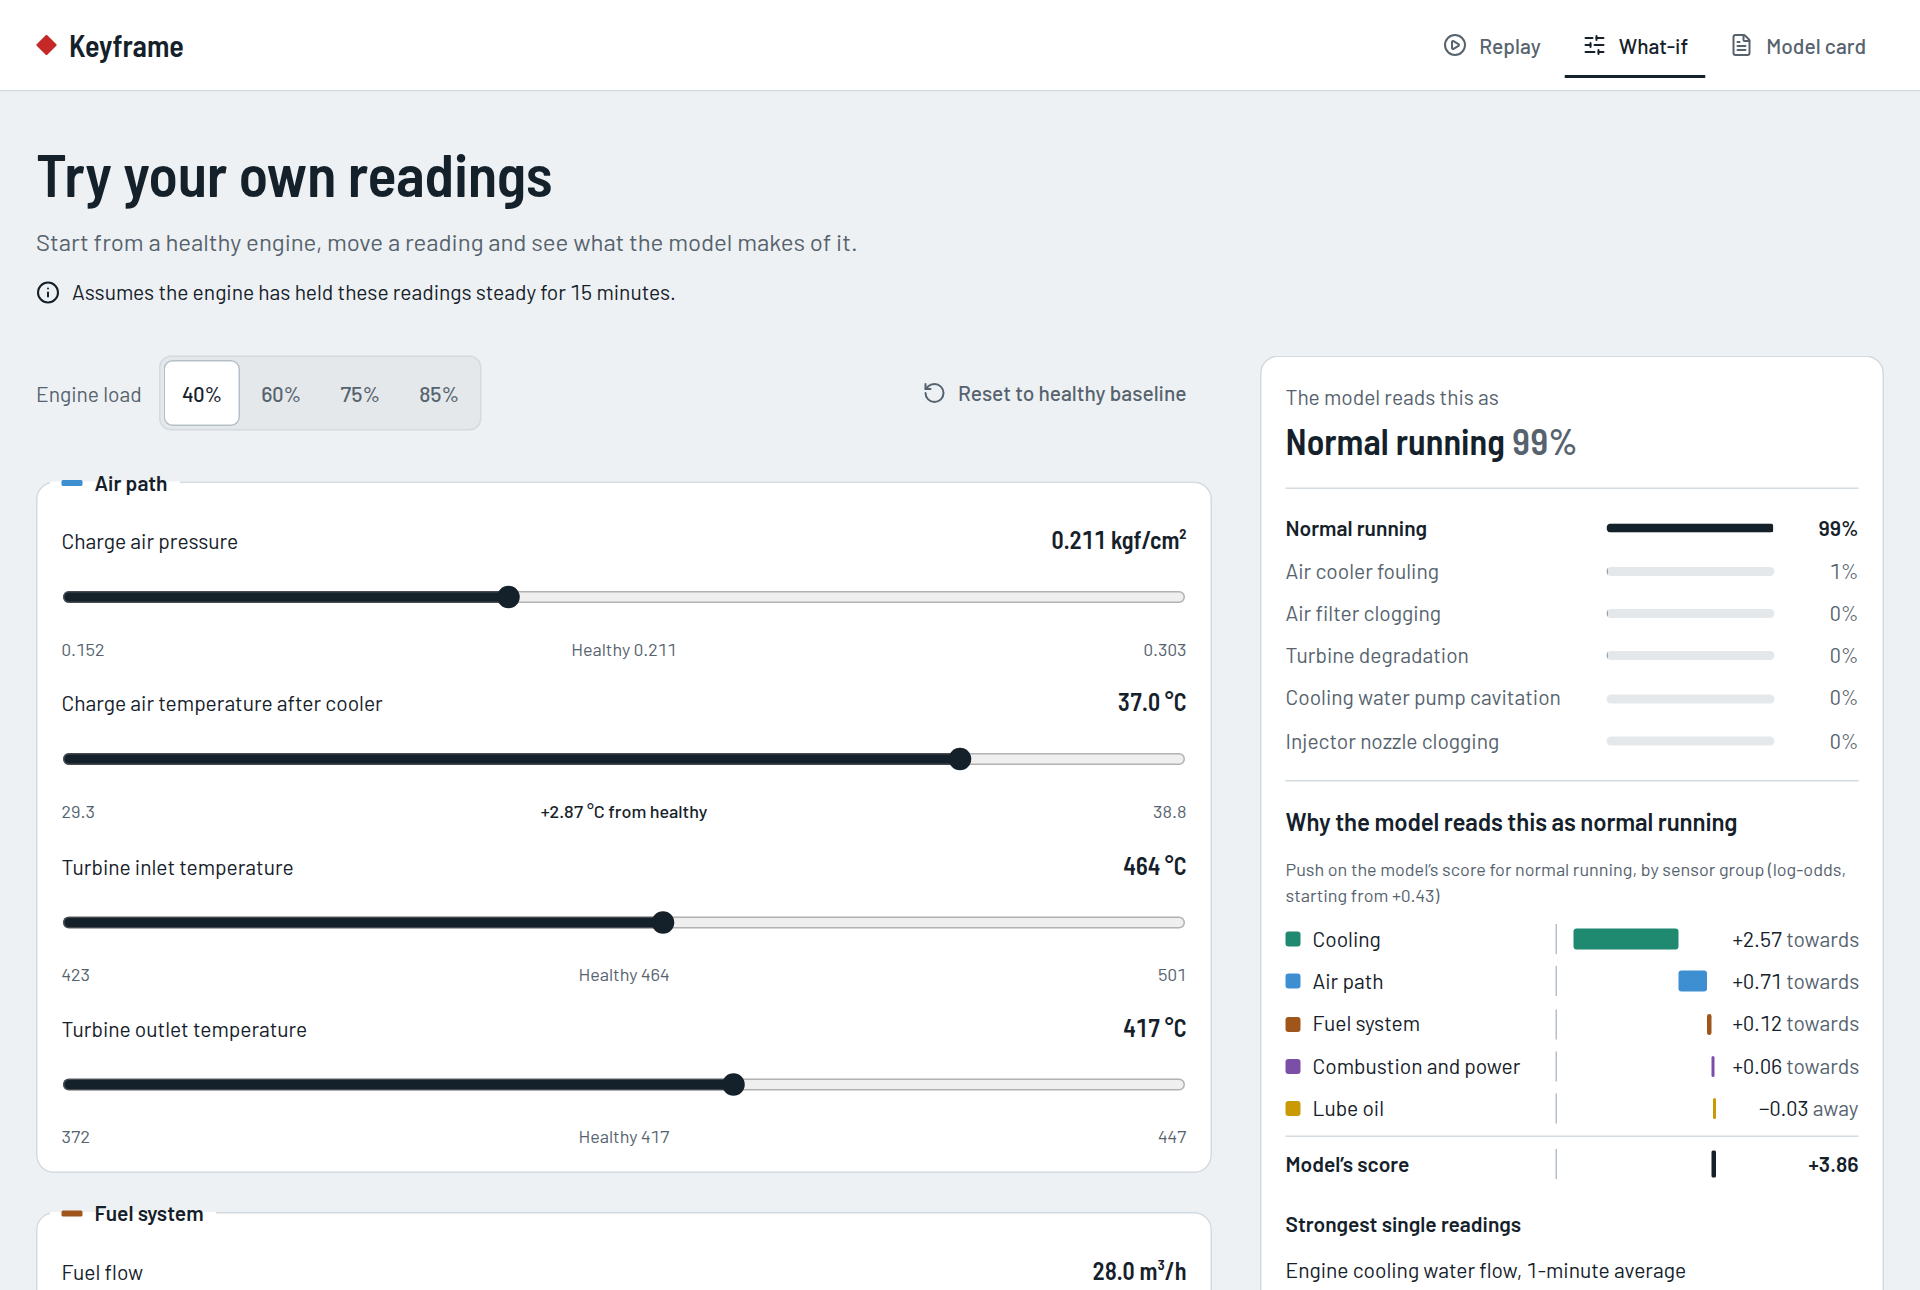
\includegraphics[width=\linewidth]{ui-whatif}
\caption{What-if: readings grouped by sensor group, each with its healthy value; the diagnosis beside them.}
\end{subfigure}\par\smallskip
\begin{subfigure}[t]{0.44\textwidth}\centering
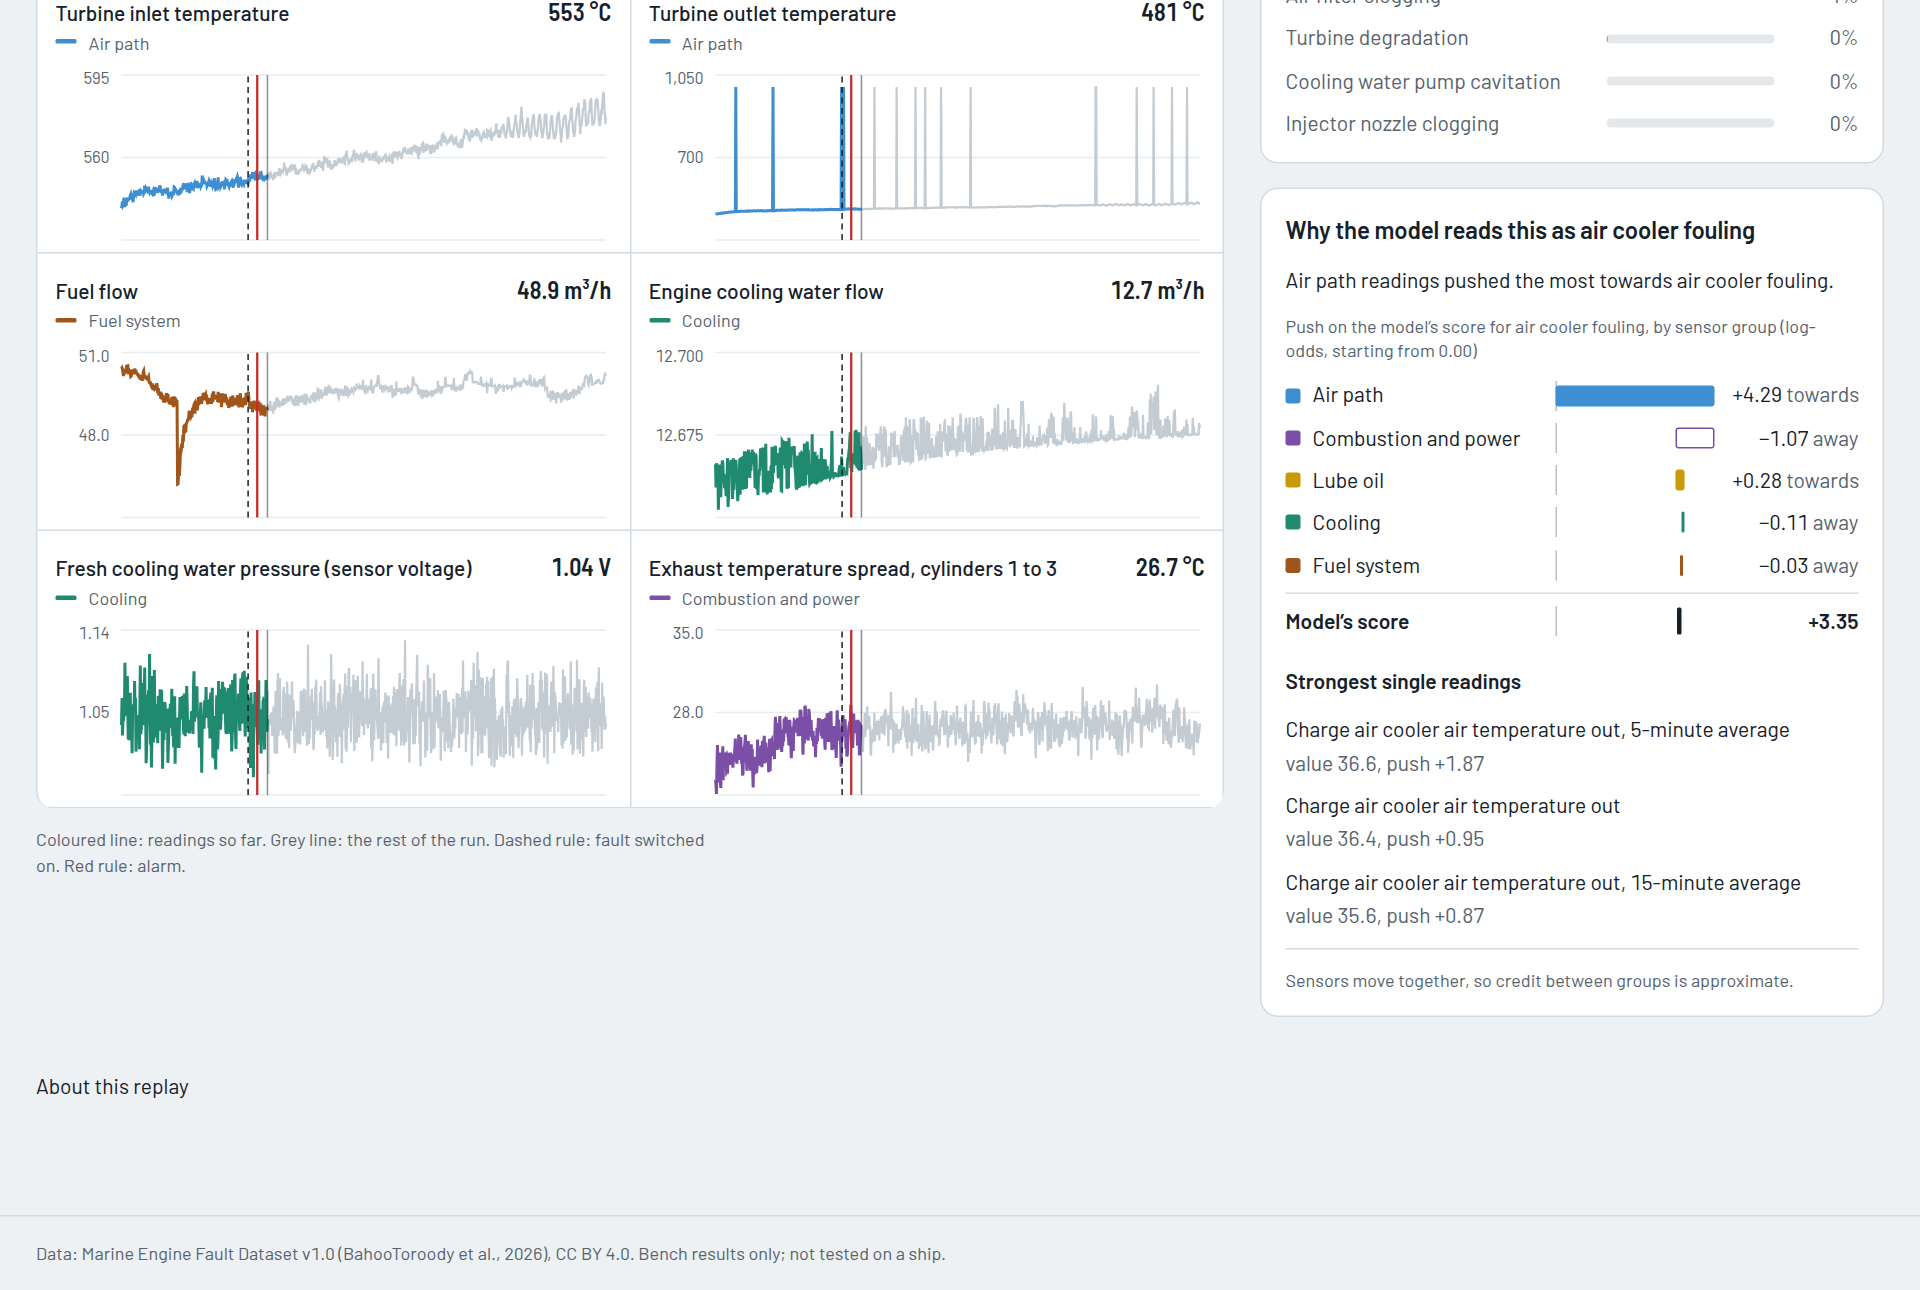
\includegraphics[width=\linewidth]{ui-explain}
\caption{Paused replay: the grouped waterfall and the strongest readings.}
\end{subfigure}\hspace{0.04\textwidth}
\begin{subfigure}[t]{0.44\textwidth}\centering
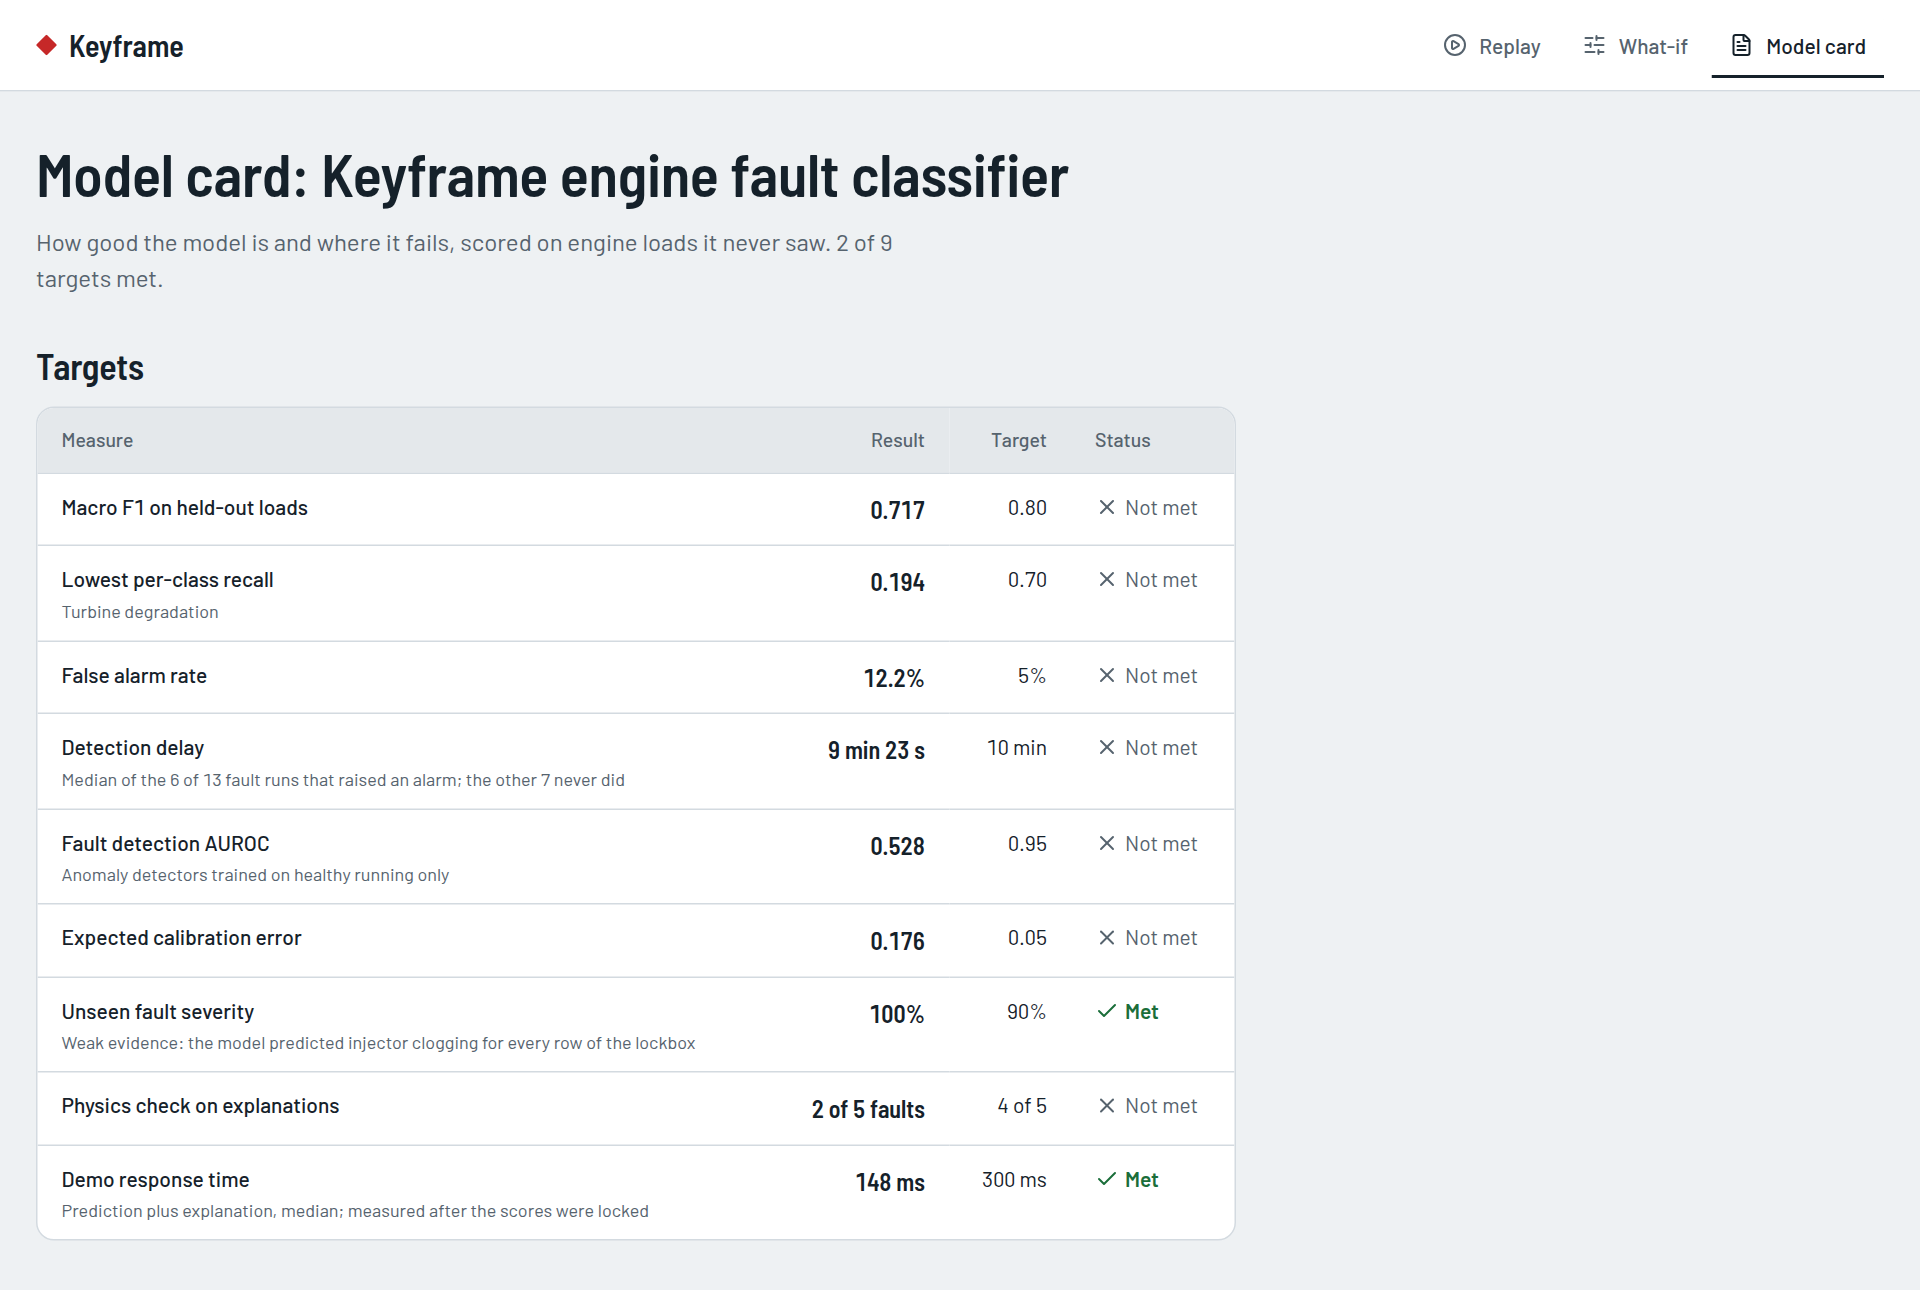
\includegraphics[width=\linewidth]{ui-modelcard}
\caption{Model card: the targets first, each with a worded status.}
\end{subfigure}
\caption{\textbf{The demo at 1280 px}, captured from the production build.}
\label{fig:ui}
\end{figure}

Writing this paper exposed a defect in the demo. The replay files had applied one alarm setting to every run, the median of the four folds' settings that the exported model uses, rather than each fold's own setting. The demo therefore showed alarms on 9 of 13 fault runs where the evaluation found \AlarmDetected, and the median itself drew on settings chosen with the replayed load in their training data. The replays now use each fold's own setting, and a test holds every replay's alarm delay to the evaluated one, allowing only the 10-second frame thinning. The exported model keeps the median setting (\ExportAlarmDuration\,s at probability \ExportAlarmProbability) as a deployment choice with no held-out score of its own.

% ==============================================================================
\section{Verification}
% ==============================================================================

The project was built feature by feature from a written brief. Each feature had requirements, validation checks and small tickets, and each ticket had to pass lint, formatting, type checks and the tests before it was committed. Decisions the brief did not settle are recorded in twelve decision records.

\begin{itemize}
  \item \textbf{Python tests} (pytest, \TestsPython{} tests): data loading and the audit, splits that never mix engine loads, causal rolling windows, residual models fitted on training rows only, the alarm logic, metrics, the pinned checklist hash, the lockbox scored only by an explicit first run and never refitted, the exported model reproducing a stored prediction in a clean session, API latency, and replay alarms matching the evaluation.
  \item \textbf{Web tests} (Vitest, \TestsWeb{} tests): playback, the timeline scrubber and keyboard controls, formatting of readings, every view's states, colour tokens, and the demo's targets table checked against the results files.
  \item \textbf{Generated numbers}: this paper's numbers, tables and plot data are written by one script from the results files, and a test checks that the committed copies match a fresh run.
  \item \textbf{Reproduction}: one script rebuilds every experiment, notebook, figure and demo file from a fresh clone, in the order they were made.
\end{itemize}

% ==============================================================================
\section{Limitations}
% ==============================================================================

The data come from one small engine on a test bench at steady loads, with \DataFaultRuns{} fault runs; turbine degradation and cavitation have only three and two. The model has not been tested on a ship and must not be used for operating or maintenance decisions. Scores vary strongly between held-out loads, and with one run per fault and load, a single run can move a fold's score. Part of the score for air filter clogging and cavitation comes from recognising the test day. Confidence is not calibrated. The 85\,\% fold's model is underfit, and the tuning budget allowed only a handful of trials per fold; a better-tuned version would have to be reported as a new evaluation, not as a replacement. The explanations are SHAP values of a model fitted to correlated sensors, and only two faults' explanations agree with the physics.

% ==============================================================================
\section{Conclusion}
% ==============================================================================

On real bench data and a load it never saw, a gradient-boosted classifier diagnoses injector clogging and air cooler fouling from the readings an engineer would look at, raises a correct sustained alarm for four of the five faults in at least one run, and does so in \AlarmDetected{} of \AlarmRuns{} fault runs. It misses most of its targets, and part of its score for two faults comes from the test day rather than the fault. Setting the targets, the checklist and the lockbox aside before modelling made those findings visible instead of hiding them behind a random split. Generating the paper from the results files also exposed a real defect, demo alarms computed with the wrong settings, which is now fixed and guarded by a test.

\paragraph{Data and code.} The dataset is by BahooToroody et al.~\cite{bahootoroody2026dataset,bahootoroody2026descriptor}, released under CC BY 4.0. The code, notebooks, results and demo are in the \kf{} repository.

\bibliographystyle{plainnat}
\bibliography{references}

\end{document}
